\documentclass[tikz,border=10pt]{standalone}
\usepackage{tikz}
\usepackage{amsmath}
\usepackage{xcolor}
\usetikzlibrary{shapes,arrows,positioning,calc}

% Define colors
\definecolor{layer1}{RGB}{230, 240, 255}   % User Interface Layer
\definecolor{layer2}{RGB}{210, 255, 210}   % Application Layer
\definecolor{layer3}{RGB}{255, 240, 200}   % Processing Layer
\definecolor{layer4}{RGB}{255, 220, 220}   % Infrastructure Layer
\definecolor{quantum}{RGB}{0, 100, 200}
\definecolor{aicolor}{RGB}{0, 150, 0}
\definecolor{blockchain}{RGB}{200, 80, 0}
\definecolor{dataflow}{RGB}{100, 100, 100}

\begin{document}
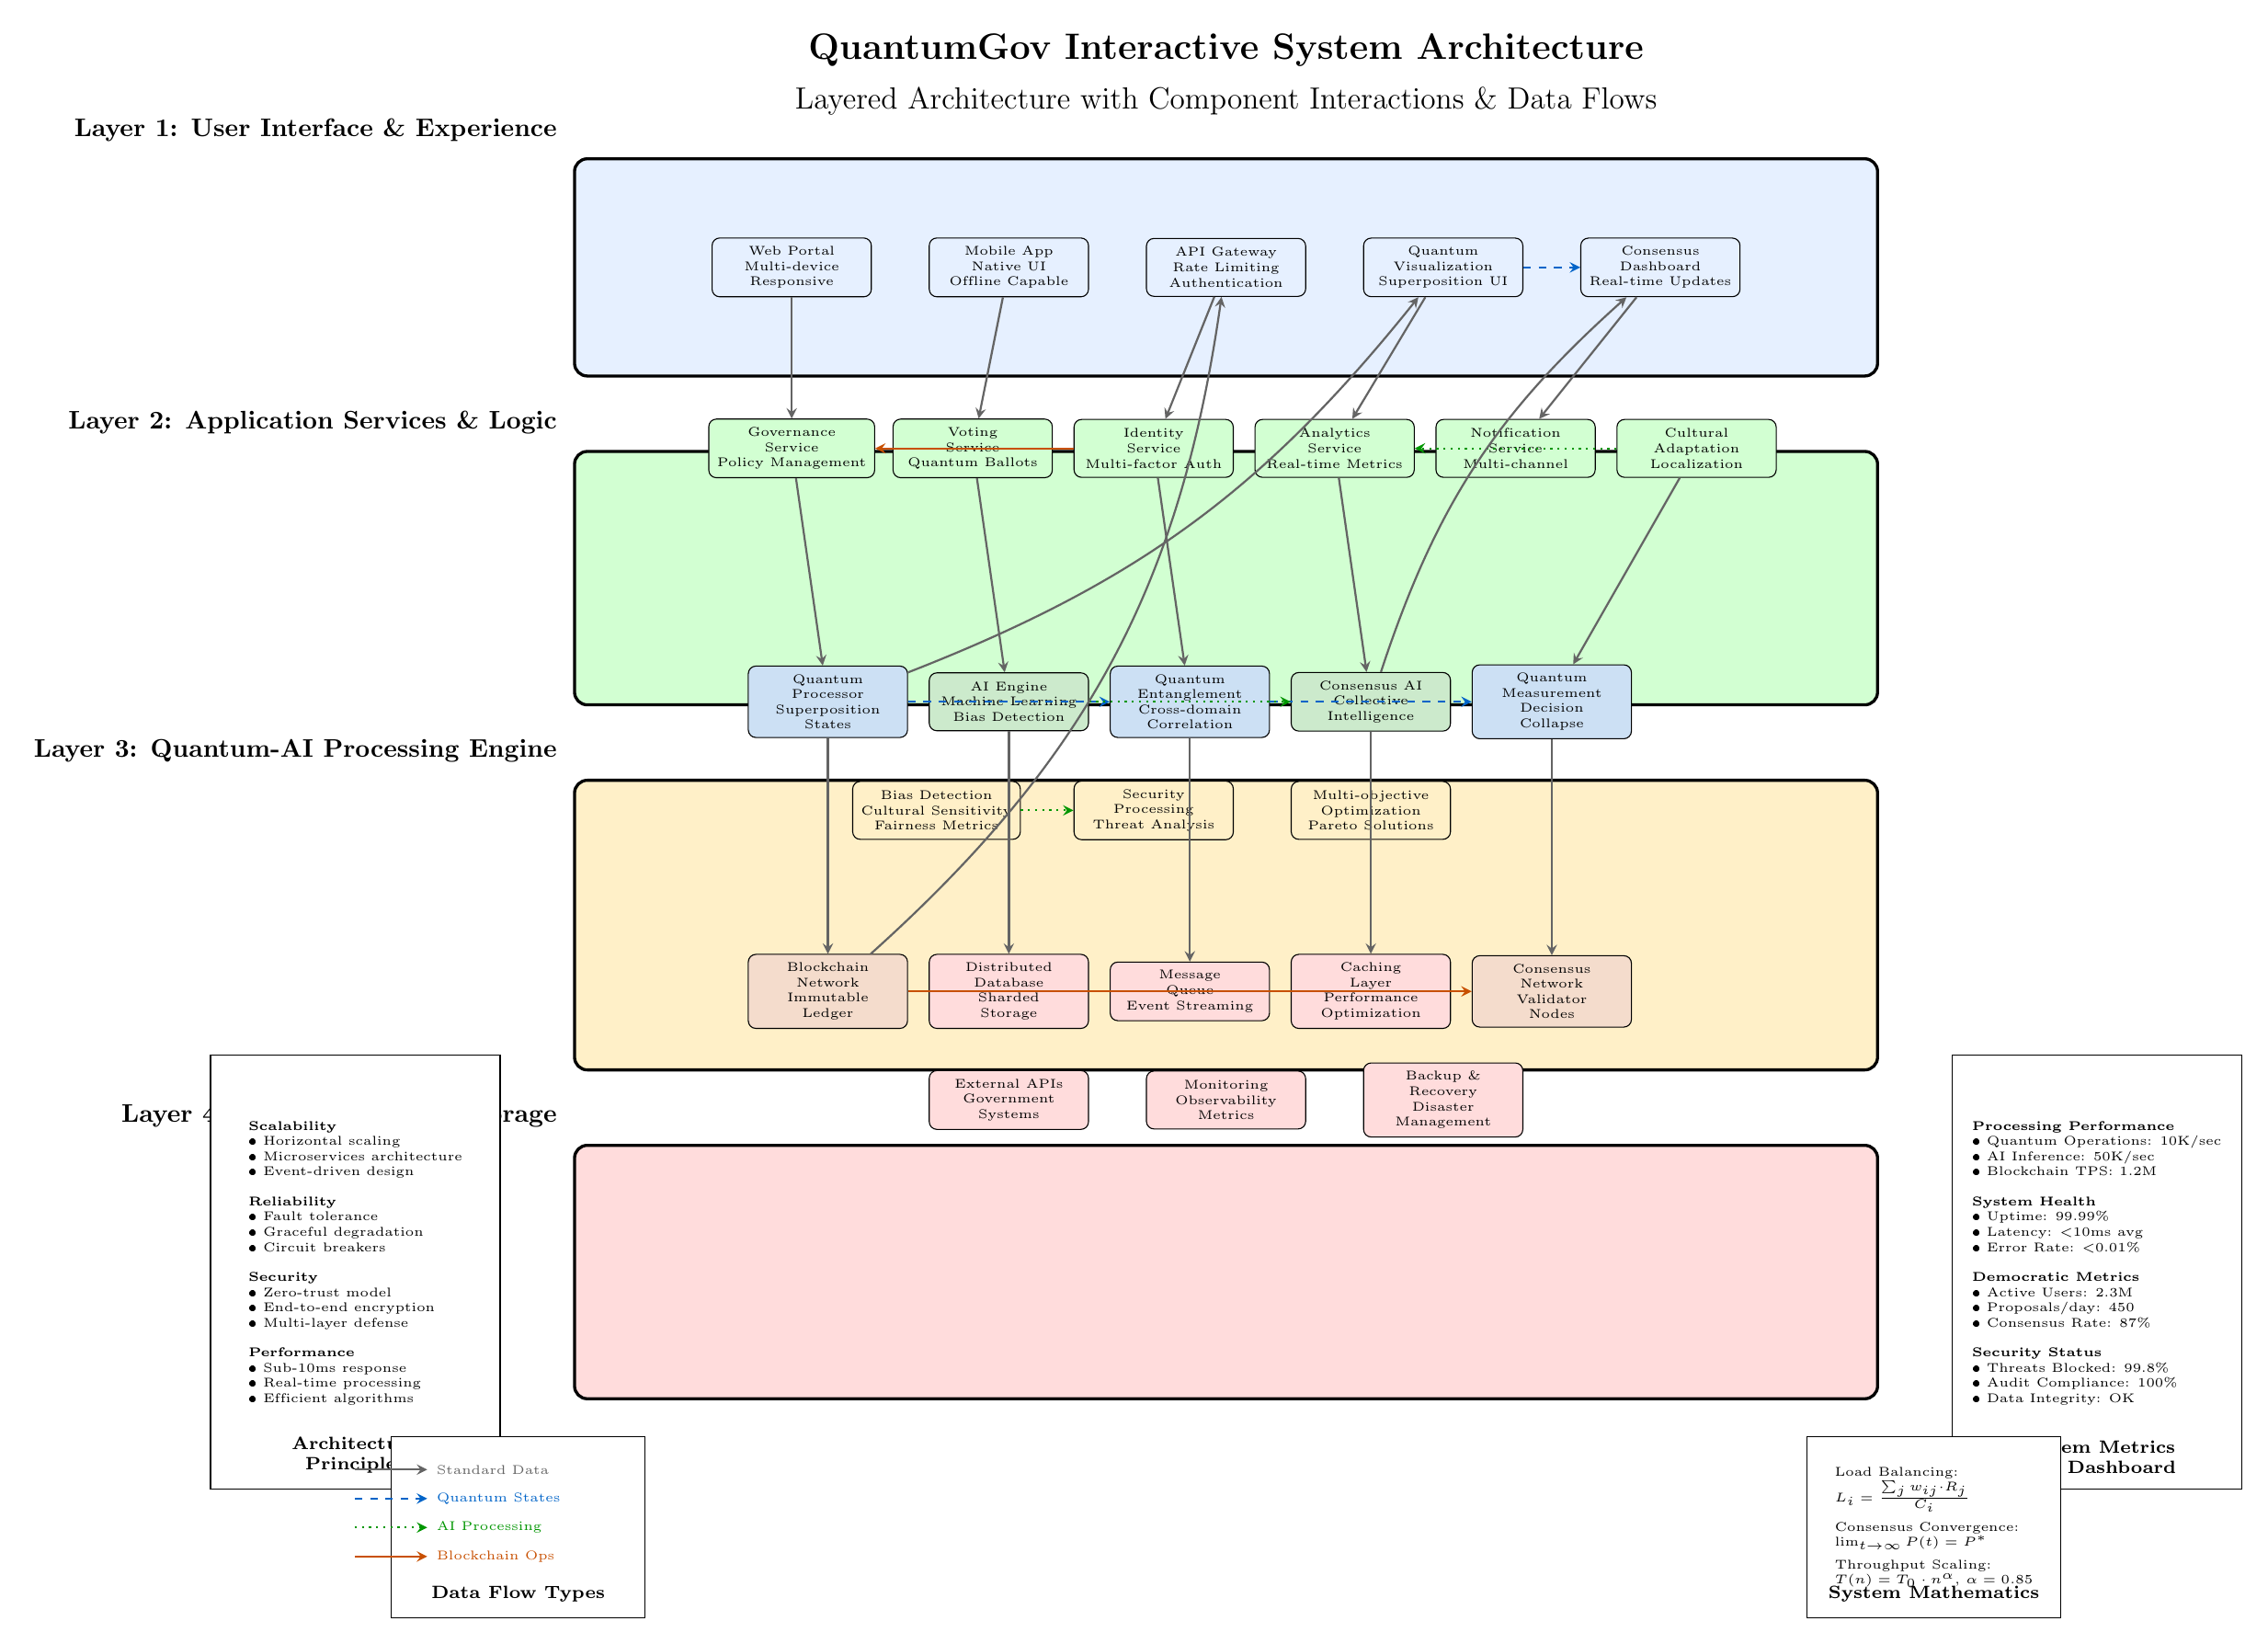
\begin{tikzpicture}[
    node distance=0.8cm,
    component/.style={rectangle, rounded corners=3pt, draw, minimum height=0.8cm, minimum width=2.2cm, align=center, font=\tiny},
    layer/.style={rectangle, rounded corners=5pt, draw, very thick, minimum height=3cm, align=center},
    dataflow/.style={->, thick, color=dataflow, >=stealth},
    quantum_flow/.style={->, thick, color=quantum, >=stealth, dashed},
    ai_flow/.style={->, thick, color=aicolor, >=stealth, dotted},
    blockchain_flow/.style={->, thick, color=blockchain, >=stealth}
]

% Title
\node[align=center, font=\Large\bfseries] at (0, 16) {QuantumGov Interactive System Architecture};
\node[align=center, font=\large] at (0, 15.3) {Layered Architecture with Component Interactions \& Data Flows};

% Layer 1: User Interface Layer
\node[layer, fill=layer1, minimum width=18cm, minimum height=3cm] (ui_layer) at (0, 13) {};
\node[above left=0.1cm and 0.1cm of ui_layer.north west, font=\bfseries] {Layer 1: User Interface \& Experience};

% UI Components
\node[component, fill=layer1] (web_ui) at (-6, 13) {Web Portal\\Multi-device\\Responsive};
\node[component, fill=layer1] (mobile_ui) at (-3, 13) {Mobile App\\Native UI\\Offline Capable};
\node[component, fill=layer1] (api_gateway) at (0, 13) {API Gateway\\Rate Limiting\\Authentication};
\node[component, fill=layer1] (quantum_viz) at (3, 13) {Quantum\\Visualization\\Superposition UI};
\node[component, fill=layer1] (consensus_ui) at (6, 13) {Consensus\\Dashboard\\Real-time Updates};

% Layer 2: Application Layer
\node[layer, fill=layer2, minimum width=18cm, minimum height=3.5cm, below=1cm of ui_layer] (app_layer) {};
\node[above left=0.1cm and 0.1cm of app_layer.north west, font=\bfseries] {Layer 2: Application Services \& Logic};

% Application Components
\node[component, fill=layer2] (gov_service) at (-6, 10.5) {Governance\\Service\\Policy Management};
\node[component, fill=layer2] (voting_service) at (-3.5, 10.5) {Voting\\Service\\Quantum Ballots};
\node[component, fill=layer2] (identity_service) at (-1, 10.5) {Identity\\Service\\Multi-factor Auth};
\node[component, fill=layer2] (analytics_service) at (1.5, 10.5) {Analytics\\Service\\Real-time Metrics};
\node[component, fill=layer2] (notification_service) at (4, 10.5) {Notification\\Service\\Multi-channel};
\node[component, fill=layer2] (cultural_service) at (6.5, 10.5) {Cultural\\Adaptation\\Localization};

% Layer 3: Processing Layer  
\node[layer, fill=layer3, minimum width=18cm, minimum height=4cm, below=1cm of app_layer] (proc_layer) {};
\node[above left=0.1cm and 0.1cm of proc_layer.north west, font=\bfseries] {Layer 3: Quantum-AI Processing Engine};

% Processing Components
\node[component, fill=quantum!20] (quantum_proc) at (-5.5, 7) {Quantum\\Processor\\Superposition\\States};
\node[component, fill=aicolor!20] (ai_engine) at (-3, 7) {AI Engine\\Machine Learning\\Bias Detection};
\node[component, fill=quantum!20] (entanglement) at (-0.5, 7) {Quantum\\Entanglement\\Cross-domain\\Correlation};
\node[component, fill=aicolor!20] (consensus_ai) at (2, 7) {Consensus AI\\Collective\\Intelligence};
\node[component, fill=quantum!20] (measurement) at (4.5, 7) {Quantum\\Measurement\\Decision\\Collapse};

% Specialized Processing
\node[component, fill=layer3] (bias_detector) at (-4, 5.5) {Bias Detection\\Cultural Sensitivity\\Fairness Metrics};
\node[component, fill=layer3] (security_proc) at (-1, 5.5) {Security\\Processing\\Threat Analysis};
\node[component, fill=layer3] (optimization) at (2, 5.5) {Multi-objective\\Optimization\\Pareto Solutions};

% Layer 4: Infrastructure Layer
\node[layer, fill=layer4, minimum width=18cm, minimum height=3.5cm, below=1cm of proc_layer] (infra_layer) {};
\node[above left=0.1cm and 0.1cm of infra_layer.north west, font=\bfseries] {Layer 4: Infrastructure \& Storage};

% Infrastructure Components
\node[component, fill=blockchain!20] (blockchain_net) at (-5.5, 3) {Blockchain\\Network\\Immutable\\Ledger};
\node[component, fill=layer4] (distributed_db) at (-3, 3) {Distributed\\Database\\Sharded\\Storage};
\node[component, fill=layer4] (message_queue) at (-0.5, 3) {Message\\Queue\\Event Streaming};
\node[component, fill=layer4] (cache_layer) at (2, 3) {Caching\\Layer\\Performance\\Optimization};
\node[component, fill=blockchain!20] (consensus_net) at (4.5, 3) {Consensus\\Network\\Validator\\Nodes};

% External Integrations
\node[component, fill=layer4] (ext_apis) at (-3, 1.5) {External APIs\\Government\\Systems};
\node[component, fill=layer4] (monitoring) at (0, 1.5) {Monitoring\\Observability\\Metrics};
\node[component, fill=layer4] (backup) at (3, 1.5) {Backup \&\\Recovery\\Disaster\\Management};

% Data Flow Arrows - Vertical
\draw[dataflow] (web_ui) -- (gov_service);
\draw[dataflow] (mobile_ui) -- (voting_service);
\draw[dataflow] (api_gateway) -- (identity_service);
\draw[dataflow] (quantum_viz) -- (analytics_service);
\draw[dataflow] (consensus_ui) -- (notification_service);

\draw[dataflow] (gov_service) -- (quantum_proc);
\draw[dataflow] (voting_service) -- (ai_engine);
\draw[dataflow] (identity_service) -- (entanglement);
\draw[dataflow] (analytics_service) -- (consensus_ai);
\draw[dataflow] (cultural_service) -- (measurement);

\draw[dataflow] (quantum_proc) -- (blockchain_net);
\draw[dataflow] (ai_engine) -- (distributed_db);
\draw[dataflow] (entanglement) -- (message_queue);
\draw[dataflow] (consensus_ai) -- (cache_layer);
\draw[dataflow] (measurement) -- (consensus_net);

% Horizontal Data Flows - Quantum
\draw[quantum_flow] (quantum_proc) -- (entanglement);
\draw[quantum_flow] (entanglement) -- (measurement);
\draw[quantum_flow] (quantum_viz) -- (consensus_ui);

% Horizontal Data Flows - AI
\draw[ai_flow] (ai_engine) -- (consensus_ai);
\draw[ai_flow] (bias_detector) -- (security_proc);
\draw[ai_flow] (cultural_service) -- (analytics_service);

% Horizontal Data Flows - Blockchain
\draw[blockchain_flow] (blockchain_net) -- (consensus_net);
\draw[blockchain_flow] (identity_service) -- (gov_service);

% Cross-layer connections
\draw[dataflow, bend right=15] (quantum_proc) to (quantum_viz);
\draw[dataflow, bend left=15] (consensus_ai) to (consensus_ui);
\draw[dataflow, bend right=20] (blockchain_net) to (api_gateway);

% Performance Metrics Panel
\node[draw, fill=white, minimum width=4cm, minimum height=6cm, right=1cm of infra_layer] (metrics_panel) {};
\node[above=0.1cm of metrics_panel.south, font=\scriptsize\bfseries, align=center] {System Metrics\\Live Dashboard};
\node[below=0.8cm of metrics_panel.north, font=\tiny, align=left] {
    \textbf{Processing Performance}\\
    • Quantum Operations: 10K/sec\\
    • AI Inference: 50K/sec\\
    • Blockchain TPS: 1.2M\\[0.2cm]
    \textbf{System Health}\\
    • Uptime: 99.99\%\\
    • Latency: <10ms avg\\
    • Error Rate: <0.01\%\\[0.2cm]
    \textbf{Democratic Metrics}\\
    • Active Users: 2.3M\\
    • Proposals/day: 450\\
    • Consensus Rate: 87\%\\[0.2cm]
    \textbf{Security Status}\\
    • Threats Blocked: 99.8\%\\
    • Audit Compliance: 100\%\\
    • Data Integrity: OK
};

% Architecture Principles Panel
\node[draw, fill=white, minimum width=4cm, minimum height=6cm, left=1cm of infra_layer] (principles_panel) {};
\node[above=0.1cm of principles_panel.south, font=\scriptsize\bfseries, align=center] {Architecture\\Principles};
\node[below=0.8cm of principles_panel.north, font=\tiny, align=left] {
    \textbf{Scalability}\\
    • Horizontal scaling\\
    • Microservices architecture\\
    • Event-driven design\\[0.2cm]
    \textbf{Reliability}\\
    • Fault tolerance\\
    • Graceful degradation\\
    • Circuit breakers\\[0.2cm]
    \textbf{Security}\\
    • Zero-trust model\\
    • End-to-end encryption\\
    • Multi-layer defense\\[0.2cm]
    \textbf{Performance}\\
    • Sub-10ms response\\
    • Real-time processing\\
    • Efficient algorithms
};

% Data Flow Legend
\node[draw, fill=white, minimum width=3.5cm, minimum height=2.5cm, below left=0.5cm and -1cm of infra_layer] (legend) {};
\node[above=0.1cm of legend.south, font=\scriptsize\bfseries, align=center] {Data Flow Types};
\draw[dataflow] (legend.west) ++(-0.5, 0.8) -- ++(1, 0) node[right, font=\tiny] {Standard Data};
\draw[quantum_flow] (legend.west) ++(-0.5, 0.4) -- ++(1, 0) node[right, font=\tiny] {Quantum States};
\draw[ai_flow] (legend.west) ++(-0.5, 0) -- ++(1, 0) node[right, font=\tiny] {AI Processing};
\draw[blockchain_flow] (legend.west) ++(-0.5, -0.4) -- ++(1, 0) node[right, font=\tiny] {Blockchain Ops};

% Mathematical Framework
\node[draw, fill=white, minimum width=3.5cm, minimum height=2.5cm, below right=0.5cm and -1cm of infra_layer] (math_framework) {};
\node[above=0.1cm of math_framework.south, font=\scriptsize\bfseries, align=center] {System Mathematics};
\node[below=0.3cm of math_framework.north, font=\tiny, align=left] {
    Load Balancing:\\
    $L_i = \frac{\sum_{j} w_{ij} \cdot R_j}{C_i}$\\[0.1cm]
    Consensus Convergence:\\
    $\lim_{t \to \infty} P(t) = P^*$\\[0.1cm]
    Throughput Scaling:\\
    $T(n) = T_0 \cdot n^{\alpha}$, $\alpha = 0.85$
};

\end{tikzpicture}
\end{document}